\documentclass{article}
\usepackage[x11names, svgnames, rgb]{xcolor}
\usepackage[utf8]{inputenc}
\usepackage{tikz}
\usetikzlibrary{snakes,arrows,shapes}
\usepackage{amsmath}
%
%

%

%

\begin{document}
\pagestyle{empty}
%
%
%

\enlargethispage{100cm}
% Start of code
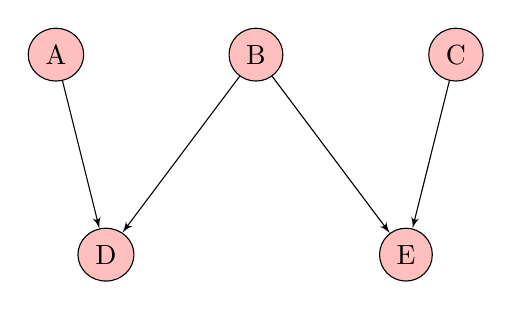
\begin{tikzpicture}[>=latex',line join=bevel,]
%%
\node (A) at (27.0bp,90.0bp) [draw,fill=pink,ellipse] {A};
  \node (D) at (45.0bp,18.0bp) [draw,fill=pink,ellipse] {D};
  \node (B) at (99.0bp,90.0bp) [draw,fill=pink,ellipse] {B};
  \node (E) at (153.0bp,18.0bp) [draw,fill=pink,ellipse] {E};
  \node (C) at (171.0bp,90.0bp) [draw,fill=pink,ellipse] {C};
  \draw [->] (A) ..controls (33.44bp,64.241bp) and (35.833bp,54.667bp)  .. (D);
  \draw [->] (B) ..controls (79.842bp,64.456bp) and (71.082bp,52.776bp)  .. (D);
  \draw [->] (B) ..controls (118.16bp,64.456bp) and (126.92bp,52.776bp)  .. (E);
  \draw [->] (C) ..controls (164.56bp,64.241bp) and (162.17bp,54.667bp)  .. (E);
%
\end{tikzpicture}
% End of code

%
\end{document}
%



